\chapter{Import}
\section{Package Import}{
\label{Import}\hypertarget{Import}{}
\hskip -.05in
\hbox to \hsize{\textit{ Package Contents\hfil Page}}
\vskip .13in
\hbox{{\bf  Interfaces}}
\entityintro{FileReaderStrategy}{Import.FileReaderStrategy}{Interface for the FileReaderStrategy classes.}
\vskip .13in
\hbox{{\bf  Classes}}
\entityintro{CSVReaderStrategy}{Import.CSVReaderStrategy}{Implementation of the FileReaderStrategy interface for CSV files.}
\entityintro{DataImporter}{Import.DataImporter}{Importer for data that should be added to PaVoS.}
\entityintro{FileImporter}{Import.FileImporter}{Importer for the Data contained in a File.}
\entityintro{FrostSender}{Import.FrostSender}{sends Data to the FROST-Server.}
\entityintro{NetCDFReaderStrategy}{Import.NetCDFReaderStrategy}{Implementation of the FileReaderStrategy interface for NetCDF files.}
\entityintro{ReaderType}{Import.ReaderType}{Is like a chooser for the right FileReaderStrategy.}
\vskip .1in
\vskip .1in
\subsection{\label{Import.FileReaderStrategy}Interface FileReaderStrategy}{
\hypertarget{Import.FileReaderStrategy}{}\vskip .1in
Interface for the FileReaderStrategy classes. Realization of a Strategy to be able to swap out the way a File has to be read.\vskip .1in
\begin{figure}[!hbp]
	\centering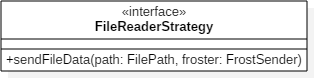
\includegraphics[width=0.5\linewidth]{images/import/classes/FileReaderStrategy}
\end{figure}
\subsubsection{Declaration}{
\begin{lstlisting}[frame=none]
public interface FileReaderStrategy
\end{lstlisting}
\subsubsection{All known subinterfaces}{NetCDFReaderStrategy\small{\refdefined{Import.NetCDFReaderStrategy}}, CSVReaderStrategy\small{\refdefined{Import.CSVReaderStrategy}}}
\subsubsection{All classes known to implement interface}{NetCDFReaderStrategy\small{\refdefined{Import.NetCDFReaderStrategy}}, CSVReaderStrategy\small{\refdefined{Import.CSVReaderStrategy}}}
\subsubsection{Method summary}{
\begin{verse}
\hyperlink{Import.FileReaderStrategy.sendFileData(FilePath, Import.FrostSender)}{{\bf sendFileData(FilePath, FrostSender)}} Reades from a File as specified by the FilePath and sends the information in it to the FROST-Server using the FrostSender that was provided.\\
\end{verse}
}
\subsubsection{Methods}{
\vskip -2em
\begin{itemize}
\item{
\index{sendFileData(FilePath, FrostSender)}
\hypertarget{Import.FileReaderStrategy.sendFileData(FilePath, Import.FrostSender)}{{\bf  sendFileData}\\}
\begin{lstlisting}[frame=none]
void sendFileData(FilePath path,FrostSender froster)\end{lstlisting} %end signature
\begin{itemize}
\item{
{\bf  Description}

Reades from a File as specified by the FilePath and sends the information in it to the FROST-Server using the FrostSender that was provided.
}
\item{
{\bf  Parameters}
  \begin{itemize}
   \item{
\texttt{path} -- Is the FilePath of the File to Import.}
   \item{
\texttt{froster} -- Is the FrostSender instance that will be used to send the files data to the Frost-Server.}
  \end{itemize}
}%end item
\end{itemize}
}%end item
\end{itemize}
}
}
\subsection{\label{Import.CSVReaderStrategy}Class CSVReaderStrategy}{
\hypertarget{Import.CSVReaderStrategy}{}\vskip .1in
Implementation of the FileReaderStrategy interface for CSV files.\vskip .1in
\begin{figure}[!hbp]
	\centering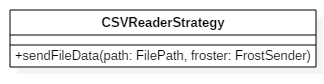
\includegraphics[width=0.5\linewidth]{images/import/classes/CSVReaderStrategy}
\end{figure}
\subsubsection{Declaration}{
\begin{lstlisting}[frame=none]
public class CSVReaderStrategy
 extends java.lang.Object implements FileReaderStrategy\end{lstlisting}
\subsubsection{Constructor summary}{
\begin{verse}
\hyperlink{Import.CSVReaderStrategy()}{{\bf CSVReaderStrategy()}} Default constructor\\
\end{verse}
}
\subsubsection{Method summary}{
\begin{verse}
\hyperlink{Import.CSVReaderStrategy.sendFileData(FilePath, Import.FrostSender)}{{\bf sendFileData(FilePath, FrostSender)}} Reades from a File as specified by the FilePath and sends the information in it to the FROST-Server using the FrostSender that was provided.\\
\hyperlink{Import.CSVReaderStrategy.sendFileData(FilePath, Import.FrostSender)}{{\bf sendFileData(FilePath, FrostSender)}} Reades from a File as specified by the FilePath and sends the information in it to the FROST-Server using the FrostSender that was provided.\\
\end{verse}
}
\subsubsection{Constructors}{
\vskip -2em
\begin{itemize}
\item{
\index{CSVReaderStrategy()}
\hypertarget{Import.CSVReaderStrategy()}{{\bf  CSVReaderStrategy}\\}
\begin{lstlisting}[frame=none]
public CSVReaderStrategy()\end{lstlisting} %end signature
\begin{itemize}
\item{
{\bf  Description}

Default constructor
}
\end{itemize}
}%end item
\end{itemize}
}
\subsubsection{Methods}{
\vskip -2em
\begin{itemize}
\item{
\index{sendFileData(FilePath, FrostSender)}
\hypertarget{Import.CSVReaderStrategy.sendFileData(FilePath, Import.FrostSender)}{{\bf  sendFileData}\\}
\begin{lstlisting}[frame=none]
public void sendFileData(FilePath path,FrostSender froster)\end{lstlisting} %end signature
\begin{itemize}
\item{
{\bf  Description}

Reades from a File as specified by the FilePath and sends the information in it to the FROST-Server using the FrostSender that was provided.
}
\item{
{\bf  Parameters}
  \begin{itemize}
   \item{
\texttt{path} -- Is the FilePath of the File to Import.}
   \item{
\texttt{froster} -- Is the FrostSender instance that will be used to send the files data to the Frost-Server.}
  \end{itemize}
}%end item
\end{itemize}
}%end item
\item{
\index{sendFileData(FilePath, FrostSender)}
\hypertarget{Import.CSVReaderStrategy.sendFileData(FilePath, Import.FrostSender)}{{\bf  sendFileData}\\}
\begin{lstlisting}[frame=none]
public void sendFileData(FilePath path,FrostSender froster)\end{lstlisting} %end signature
\begin{itemize}
\item{
{\bf  Description}

Reades from a File as specified by the FilePath and sends the information in it to the FROST-Server using the FrostSender that was provided.
}
\item{
{\bf  Parameters}
  \begin{itemize}
   \item{
\texttt{path} -- Is the FilePath of the File to Import.}
   \item{
\texttt{froster} -- Is the FrostSender instance that will be used to send the files data to the Frost-Server.}
  \end{itemize}
}%end item
\end{itemize}
}%end item
\end{itemize}
}
}
\subsection{\label{Import.DataImporter}Class DataImporter}{
\hypertarget{Import.DataImporter}{}\vskip .1in
Importer for data that should be added to PaVoS. Import takes place for files in a specified folder of the server.\vskip .1in
\begin{figure}[!hbp]
	\centering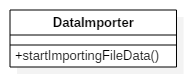
\includegraphics[width=0.4\linewidth]{images/import/classes/DataImporter}
\end{figure}
\subsubsection{Declaration}{
\begin{lstlisting}[frame=none]
public class DataImporter
 extends java.lang.Object\end{lstlisting}
\subsubsection{Constructor summary}{
\begin{verse}
\hyperlink{Import.DataImporter()}{{\bf DataImporter()}} Default constructor\\
\end{verse}
}
\subsubsection{Method summary}{
\begin{verse}
\hyperlink{Import.DataImporter.startImportingFileData()}{{\bf startImportingFileData()}} Checks for files in the specified import folder and opens a new thread for each of them, where a FileImporter is started to import the contained data.\\
\end{verse}
}
\subsubsection{Constructors}{
\vskip -2em
\begin{itemize}
\item{
\index{DataImporter()}
\hypertarget{Import.DataImporter()}{{\bf  DataImporter}\\}
\begin{lstlisting}[frame=none]
public DataImporter()\end{lstlisting} %end signature
\begin{itemize}
\item{
{\bf  Description}

Default constructor
}
\end{itemize}
}%end item
\end{itemize}
}
\subsubsection{Methods}{
\vskip -2em
\begin{itemize}
\item{
\index{startImportingFileData()}
\hypertarget{Import.DataImporter.startImportingFileData()}{{\bf  startImportingFileData}\\}
\begin{lstlisting}[frame=none]
public void startImportingFileData()\end{lstlisting} %end signature
\begin{itemize}
\item{
{\bf  Description}

Checks for files in the specified import folder and opens a new thread for each of them, where a FileImporter is started to import the contained data.
}
\end{itemize}
}%end item
\end{itemize}
}
}
\subsection{\label{Import.FileImporter}Class FileImporter}{
\hypertarget{Import.FileImporter}{}\vskip .1in
Importer for the Data contained in a File. Takes the Data and sends them to the FROST-Server.\vskip .1in
\begin{figure}[!hbp]
	\centering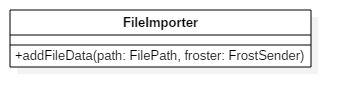
\includegraphics[width=0.5\linewidth]{images/import/classes/FileImporter}
\end{figure}
\subsubsection{Declaration}{
\begin{lstlisting}[frame=none]
public class FileImporter
 extends java.lang.Object\end{lstlisting}
\subsubsection{Constructor summary}{
\begin{verse}
\hyperlink{Import.FileImporter()}{{\bf FileImporter()}} Default constructor\\
\end{verse}
}
\subsubsection{Method summary}{
\begin{verse}
\hyperlink{Import.FileImporter.addFileData(FilePath, Import.FrostSender)}{{\bf addFileData(FilePath, FrostSender)}} Adds the Data of a File at a specified FilePath to the FROST-Server.\\
\end{verse}
}
\subsubsection{Constructors}{
\vskip -2em
\begin{itemize}
\item{
\index{FileImporter()}
\hypertarget{Import.FileImporter()}{{\bf  FileImporter}\\}
\begin{lstlisting}[frame=none]
public FileImporter()\end{lstlisting} %end signature
\begin{itemize}
\item{
{\bf  Description}

Default constructor
}
\end{itemize}
}%end item
\end{itemize}
}
\subsubsection{Methods}{
\vskip -2em
\begin{itemize}
\item{
\index{addFileData(FilePath, FrostSender)}
\hypertarget{Import.FileImporter.addFileData(FilePath, Import.FrostSender)}{{\bf  addFileData}\\}
\begin{lstlisting}[frame=none]
public void addFileData(FilePath path,FrostSender froster)\end{lstlisting} %end signature
\begin{itemize}
\item{
{\bf  Description}

Adds the Data of a File at a specified FilePath to the FROST-Server. To do so, the FileExtension of the File is determined.With help of the readerTypeClass the matching implementation of the FileReaderStrategy interface for the FileExtension is generated and can be used to get the Data from then File.
}
\item{
{\bf  Parameters}
  \begin{itemize}
   \item{
\texttt{path} -- Is the FilePath of the File to Import.}
   \item{
\texttt{froster} -- Is the FrostSender instance that will be used to send the files data to the Frost-Server.}
  \end{itemize}
}%end item
\end{itemize}
}%end item
\end{itemize}
}
}
\subsection{\label{Import.FrostSender}Class FrostSender}{
\hypertarget{Import.FrostSender}{}\vskip .1in
sends Data to the FROST-Server.\vskip .1in
\begin{figure}[!hbp]
	\centering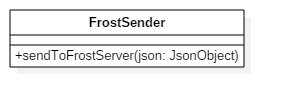
\includegraphics[width=0.5\linewidth]{images/import/classes/FrostSender}
\end{figure}
\subsubsection{Declaration}{
\begin{lstlisting}[frame=none]
public class FrostSender
 extends java.lang.Object\end{lstlisting}
\subsubsection{Constructor summary}{
\begin{verse}
\hyperlink{Import.FrostSender()}{{\bf FrostSender()}} Default constructor\\
\end{verse}
}
\subsubsection{Method summary}{
\begin{verse}
\hyperlink{Import.FrostSender.sendToFrostServer(JsonObject)}{{\bf sendToFrostServer(JsonObject)}} Sends the given JsonObject to the FROST-Server.\\
\end{verse}
}
\subsubsection{Constructors}{
\vskip -2em
\begin{itemize}
\item{
\index{FrostSender()}
\hypertarget{Import.FrostSender()}{{\bf  FrostSender}\\}
\begin{lstlisting}[frame=none]
public FrostSender()\end{lstlisting} %end signature
\begin{itemize}
\item{
{\bf  Description}

Default constructor
}
\end{itemize}
}%end item
\end{itemize}
}
\subsubsection{Methods}{
\vskip -2em
\begin{itemize}
\item{
\index{sendToFrostServer(JsonObject)}
\hypertarget{Import.FrostSender.sendToFrostServer(JsonObject)}{{\bf  sendToFrostServer}\\}
\begin{lstlisting}[frame=none]
public void sendToFrostServer(JsonObject json)\end{lstlisting} %end signature
\begin{itemize}
\item{
{\bf  Description}

Sends the given JsonObject to the FROST-Server.
}
\item{
{\bf  Parameters}
  \begin{itemize}
   \item{
\texttt{json} -- Represents a single ObservedProperty.}
  \end{itemize}
}%end item
\end{itemize}
}%end item
\end{itemize}
}
}
\subsection{\label{Import.NetCDFReaderStrategy}Class NetCDFReaderStrategy}{
\hypertarget{Import.NetCDFReaderStrategy}{}\vskip .1in
Implementation of the FileReaderStrategy interface for NetCDF files.\vskip .1in
\begin{figure}[!hbp]
	\centering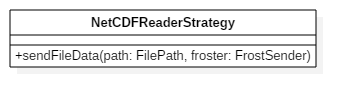
\includegraphics[width=0.5\linewidth]{images/import/classes/NetCDFReaderStrategy}
\end{figure}
\subsubsection{Declaration}{
\begin{lstlisting}[frame=none]
public class NetCDFReaderStrategy
 extends java.lang.Object implements FileReaderStrategy\end{lstlisting}
\subsubsection{Constructor summary}{
\begin{verse}
\hyperlink{Import.NetCDFReaderStrategy()}{{\bf NetCDFReaderStrategy()}} Default constructor\\
\end{verse}
}
\subsubsection{Method summary}{
\begin{verse}
\hyperlink{Import.NetCDFReaderStrategy.sendFileData(FilePath, Import.FrostSender)}{{\bf sendFileData(FilePath, FrostSender)}} Reades from a File as specified by the FilePath and sends the information in it to the FROST-Server using the FrostSender that was provided.\\
\hyperlink{Import.NetCDFReaderStrategy.sendFileData(FilePath, Import.FrostSender)}{{\bf sendFileData(FilePath, FrostSender)}} Reades from a File as specified by the FilePath and sends the information in it to the FROST-Server using the FrostSender that was provided.\\
\end{verse}
}
\subsubsection{Constructors}{
\vskip -2em
\begin{itemize}
\item{
\index{NetCDFReaderStrategy()}
\hypertarget{Import.NetCDFReaderStrategy()}{{\bf  NetCDFReaderStrategy}\\}
\begin{lstlisting}[frame=none]
public NetCDFReaderStrategy()\end{lstlisting} %end signature
\begin{itemize}
\item{
{\bf  Description}

Default constructor
}
\end{itemize}
}%end item
\end{itemize}
}
\subsubsection{Methods}{
\vskip -2em
\begin{itemize}
\item{
\index{sendFileData(FilePath, FrostSender)}
\hypertarget{Import.NetCDFReaderStrategy.sendFileData(FilePath, Import.FrostSender)}{{\bf  sendFileData}\\}
\begin{lstlisting}[frame=none]
public void sendFileData(FilePath path,FrostSender froster)\end{lstlisting} %end signature
\begin{itemize}
\item{
{\bf  Description}

Reades from a File as specified by the FilePath and sends the information in it to the FROST-Server using the FrostSender that was provided.
}
\item{
{\bf  Parameters}
  \begin{itemize}
   \item{
\texttt{path} -- Is the FilePath of the File to Import.}
   \item{
\texttt{froster} -- Is the FrostSender instance that will be used to send the files data to the Frost-Server.}
  \end{itemize}
}%end item
\end{itemize}
}%end item
\item{
\index{sendFileData(FilePath, FrostSender)}
\hypertarget{Import.NetCDFReaderStrategy.sendFileData(FilePath, Import.FrostSender)}{{\bf  sendFileData}\\}
\begin{lstlisting}[frame=none]
public void sendFileData(FilePath path,FrostSender froster)\end{lstlisting} %end signature
\begin{itemize}
\item{
{\bf  Description}

Reades from a File as specified by the FilePath and sends the information in it to the FROST-Server using the FrostSender that was provided.
}
\item{
{\bf  Parameters}
  \begin{itemize}
   \item{
\texttt{path} -- Is the FilePath of the File to Import.}
   \item{
\texttt{froster} -- Is the FrostSender instance that will be used to send the files data to the Frost-Server.}
  \end{itemize}
}%end item
\end{itemize}
}%end item
\end{itemize}
}
}
\subsection{\label{Import.ReaderType}Class ReaderType}{
\hypertarget{Import.ReaderType}{}\vskip .1in
Is like a chooser for the right FileReaderStrategy. If a new Strategy is added, this class needs some changes to use the new Strategy.\vskip .1in
\begin{figure}[!hbp]
	\centering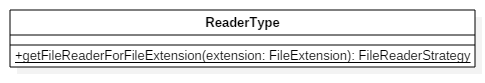
\includegraphics[width=0.6\linewidth]{images/import/classes/ReaderType}
\end{figure}
\subsubsection{Declaration}{
\begin{lstlisting}[frame=none]
public class ReaderType
 extends java.lang.Object\end{lstlisting}
\subsubsection{Constructor summary}{
\begin{verse}
\hyperlink{Import.ReaderType()}{{\bf ReaderType()}} Default constructor\\
\end{verse}
}
\subsubsection{Method summary}{
\begin{verse}
\hyperlink{Import.ReaderType.getFileReaderForFileExtension(FileExtension)}{{\bf getFileReaderForFileExtension(FileExtension)}} Gives a new Instance of a FileReaderStrategy for the specified FileExtension.\\
\end{verse}
}
\subsubsection{Constructors}{
\vskip -2em
\begin{itemize}
\item{
\index{ReaderType()}
\hypertarget{Import.ReaderType()}{{\bf  ReaderType}\\}
\begin{lstlisting}[frame=none]
public ReaderType()\end{lstlisting} %end signature
\begin{itemize}
\item{
{\bf  Description}

Default constructor
}
\end{itemize}
}%end item
\end{itemize}
}
\subsubsection{Methods}{
\vskip -2em
\begin{itemize}
\item{
\index{getFileReaderForFileExtension(FileExtension)}
\hypertarget{Import.ReaderType.getFileReaderForFileExtension(FileExtension)}{{\bf  getFileReaderForFileExtension}\\}
\begin{lstlisting}[frame=none]
public static FileReaderStrategy getFileReaderForFileExtension(FileExtension extension)\end{lstlisting} %end signature
\begin{itemize}
\item{
{\bf  Description}

Gives a new Instance of a FileReaderStrategy for the specified FileExtension.
}
\item{
{\bf  Parameters}
  \begin{itemize}
   \item{
\texttt{extension} -- is the FileExtension for which a FileReaderStrategy has to be generated.}
  \end{itemize}
}%end item
\item{{\bf  Returns} --
An instance of an implementation of the FileReaderStrategy interface.
}%end item
\end{itemize}
}%end item
\end{itemize}
}
}
}
